75. \begin{figure}[ht!]
\center{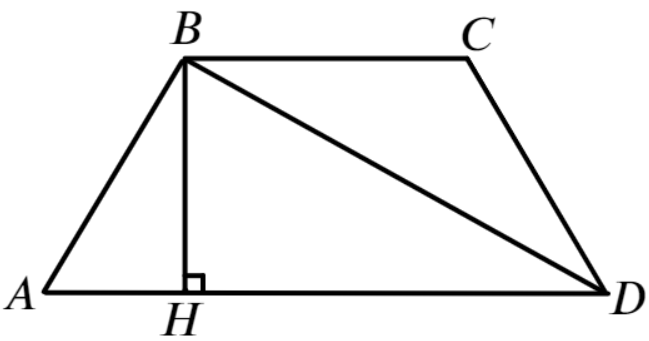
\includegraphics[scale=0.35]{g9-75.png}}
\end{figure}\\
Пусть $AB=BC=CD=1$см, $AD=2$см. Опустим высоту $BH.$ Так как трапеция равнобедренная, $AH=(2-1):2=\cfrac{1}{2},\ BH=\sqrt{1-\cfrac{1}{4}}=\cfrac{\sqrt{3}}{2}.$ Тогда $BD=\sqrt{\cfrac{3}{4}+\left(2-\cfrac{1}{2}\right)^2}=\sqrt{3}, \sin(\angle BDH)=\cfrac{\cfrac{\sqrt{3}}{2}}{\sqrt{3}}=\cfrac{1}{2}.$ Окружность, описанная вокруг трапеции $ABCD,$ описана также и вокруг треугольника $ABD,$ поэтому по теореме синусов получаем $\cfrac{AB}{\sin(\angle BDH)}=2R,\ \cfrac{1}{\cfrac{1}{2}}=2R,\ R=1$см.\\
